\chapter{绪论} 
\label{chapter:Introduction}
自从影像组学这一概念被首次提出以来\cite{lambin2012radiomics},基于医学影像组学的智能辅助诊断技术便持续成为计算机应用研究领域的研究热点\cite{lambin2012radiomics,lo2019computer}。在特定情况下,它能够为医生提供有效的决策支持,提高诊断准确性。随着数字化医学影像的广泛应用,这一技术在实际临床诊断中的需求和可控性大大增强,为深度学习在医学影像领域的落地提供了重要的突破口。这标志着智能辅助诊断技术将进一步与先进的计算机科学、机器学习相结合,为医学诊断领域带来更为准确、高效的解决方案,推动医学科技取得新的突破。

\section{研究背景及意义}
自1985年德国物理学家威廉·康拉德·伦琴(Wilhelm Conrad Röntgen)发现X射线以来\cite{bunaciu2015x},医学影像已经在医学诊断领域扮演着越来越重要的角色。在此之前,医生只能依赖解剖学来观察人体内部组织或通过确诊来了解病患身体内部的状况。然而,这种方式严重依赖医生个人经验,缺乏一致的直观和客观标准,同时存在一定的潜在风险。自20世纪50年代以来,电子科学技术的迅猛发展彻底改变了人类观察世界的方式。人们如今具备了制造精密传感器来表征各种物理量的能力。医学影像技术的崛起使得医生能够非侵入性地获得关于患者内部结构和病变的详细信息。
%X射线(X Radiography,X-Ray)\cite{warren1990x}、计算机断层扫描(Computed Tomography,CT)\cite{boyd1983cardiac}、磁共振成像(Magnetic Resonance Imaging,MRI)\cite{young1984nuclear}等高级成像技术的引入,使医生能够以前所未有的清晰度和准确性查看人体内部的各个方面。
%这一技术进步不仅提高了医学诊断的准确性,而且为医生提供了更全面的了解患者的病情,有力支持了临床决策。
随着影像技术的不断创新和进步,高清晰度影像设备(如X射线(X Radiography,X-Ray)\cite{warren1990x}、计算机断层扫描(Computed Tomography,CT)\cite{boyd1983cardiac}、磁共振成像(Magnetic Resonance Imaging,MRI)\cite{young1984nuclear}、显微影像(Microscopic Imaging,Microscopy)\cite{haider1998electron}、单光子发射计算机断层扫描(Single Photon Emission Computed Tomography,SPECT)\cite{jaszczak1980spect}、超声成像(Ultrasound,US)\cite{newman1998history}及正电子发射计算机断层扫描(Positron Emission Tomography,PET)\cite{raichle1983positron}等)的不断进步为医学诊断开辟了崭新的篇章。

%X-Ray在临床实践中的广泛应用,尤其在骨折、关节异常和肺部感染等疾病的检测方面,以其迅速而精准的成像能力为医生提供了即时的临床诊断信息。US则以其无辐射的特性,成为观察胎儿发育、腹部器官以及心脏等方面的理想检查工具,在孕妇和儿童的医疗中显示出卓越的优势。Microscopy技术通过提供高分辨率的影像,使医生能够深入观察微小结构和细胞组织,从而为疾病的早期检测和治疗提供了强大的工具。这种技术在病理学领域特别有益,可以用于癌症和其他疾病的诊断。通过显微影像,医生能够更清晰地观察组织中的细胞结构和异常,为精准的病理学评估提供支持。CT通过提供详尽的断层影像,对于复杂病变如肿瘤、血管疾病等的精准定位和评估提供了无法替代的价值。MRI则以其对软组织高分辨率的成像在神经学、心脏病学等多个领域得到广泛应用,为医生提供了更为全面的解剖信息。SPECT及PET则通过观察器官功能、代谢等方面的直观信息,对于癌症、心脏疾病等提供了关键的生物学信息。

然而,尽管这些现代医学影像设备为诊断提供了强大的支持,单一模态的影像仍存在一定的局限性,难以满足准确诊断的需求。以脑肿瘤为例,CT、MRI及PET/SPECT扫描成像差异明显,CT可以观察到脑肿瘤的硬组织结构,MRI则提供了更详细的软组织信息,而PET/SPECT则呈现了代谢活动。同样,对于阿尔茨海默病(Alzheimer's disease,AD)患者,MRI可以观察到结构性改变,而PET/SPECT则突显了代谢变化。对于帕金森疾病(Parkinson's disease,PD),DAT、DTI与PET成像也呈现不同的信息,DAT观察到神经元的损伤,DTI显示了白质纤维损害,而PET/SPECT揭示了脑部代谢活动。因此,为了得出更为全面的结论,必须结合多种影像数据或者融入临床数据(脑脊液检查、神经性评估、生物标记物检测等)进行综合分析。

另外,放射科医生在面对庞大的病例图片时,需要处理复杂的影像信息,并进行主观判断。这一判断历程容易受到医生的经验、知识储备以及疲劳程度的影响,因而存在着漏诊和误诊的潜在风险。特别是在脑部疾病的诊断过程中,如阿尔茨海默病的轻度认知障碍容易被误诊为阿尔茨海默病,帕金森疾病的早期阶段也容易被误诊为其他神经系统疾病。这些微小而关键的变化往往在诊断过程中被忽略,进一步增加了临床决策的复杂性。
随着计算机技术的不断提升和医学影像设备的普及,智能辅助诊断技术的发展为解决这些问题提供了崭新的可能性。
%这一技术的应用能够在有限的时间内精确找出支持诊断决策的影像,有效减轻医生的负担,并在一定程度上规避医生个体经验和水平对诊断结果的影响,为临床决策提供更为客观和一致的依据。
%这些创新的发展标志着医学领域正迎来一个全新的时代,其中人工智能与高清晰度影像设备相辅相成,共同推动着医学科技的演进。

    
智能辅助诊断技术利用先进的计算方法和机器学习算法,结合影像学、医学影像处理技术以及其他手段,这项技术通过分析大量数据,辅助医生在诊断过程中做出更为精确的判断,从而提高患者治疗的效果\cite{xenakis1996neglected,weiss1978model,kanthraj1997comparison,economou2001new}。该领域的开端可追溯到1950年代,那时美国学者Ledley首次将数学模型应用于临床医学领域,运用了布尔代数和Bayes定理建立计算机诊断数学模型,首次成功应用于一组肺癌病例的诊断,为智能辅助诊断技术奠定了基础。在上世纪70-80年代,智能辅助诊断系统在医学领域取得了进一步的发展,广泛用于具有明显特征的病种,如先天性心脏病、胃癌、乳腺癌等。1983年柏林举办的国际医学影像智能辅助诊断会议标志着医学影像智能辅助诊断学科的正式诞生。90年代数字化X摄影设备的普及使得数字化影像能够直接进入智能辅助诊断系统,正式进入了临床辅助医生实现智能诊断的阶段。

在21世纪的来临之际,智能辅助诊断的研究进入了全新的时代,其内容变得更加广泛与深入。随着全球医疗水平的提升,一些疾病的诊断与治疗方式得到了显著改善。与此同时,人口老龄化的趋势使得老年病逐渐成为一个备受关注的焦点,例如AD和PD等。这些疾病不仅对患者的生活和家庭构成了巨大的困扰,还会对社会经济体系产生巨大的经济压力。因此,尽早确诊对于进行有效干预、延缓病程至关重要。在这一背景下,寻找可靠而有效的疾病诊断方式显得尤为重要。本文将深入探讨了脑肿瘤、AD以及PD在影像组学的辅助下进行诊断的手段,并结合人工智能方法对疾病特征进行融合、分类与预测,提出了多种创新的辅助诊断方法。

\section{国内外研究现状}
随着科技的飞速发展,基于医学影像组学的智能辅助诊断技术正引领着医学领域的革新浪潮。在这一领域的研究,深入挖掘了传统方法与深度学习方法两大方向,呈现出多层次、多维度的探索。传统医学影像组学诊断依赖于人工设计特征和构建分类器,虽然为医生提供了一定的支持,但其在面对复杂疾病或多样化影像时表现出的局限性逐渐凸显。然而,近年来深度学习的兴起,特别是卷积神经网络的引入,赋予了模型自主学习特征的能力,显著提升了诊断性能。智能辅助诊断方面,深度学习模型的广泛应用为研究者提供了前所未有的研究机会和成果。

  \begin{figure}[htbp]
      \centering  
      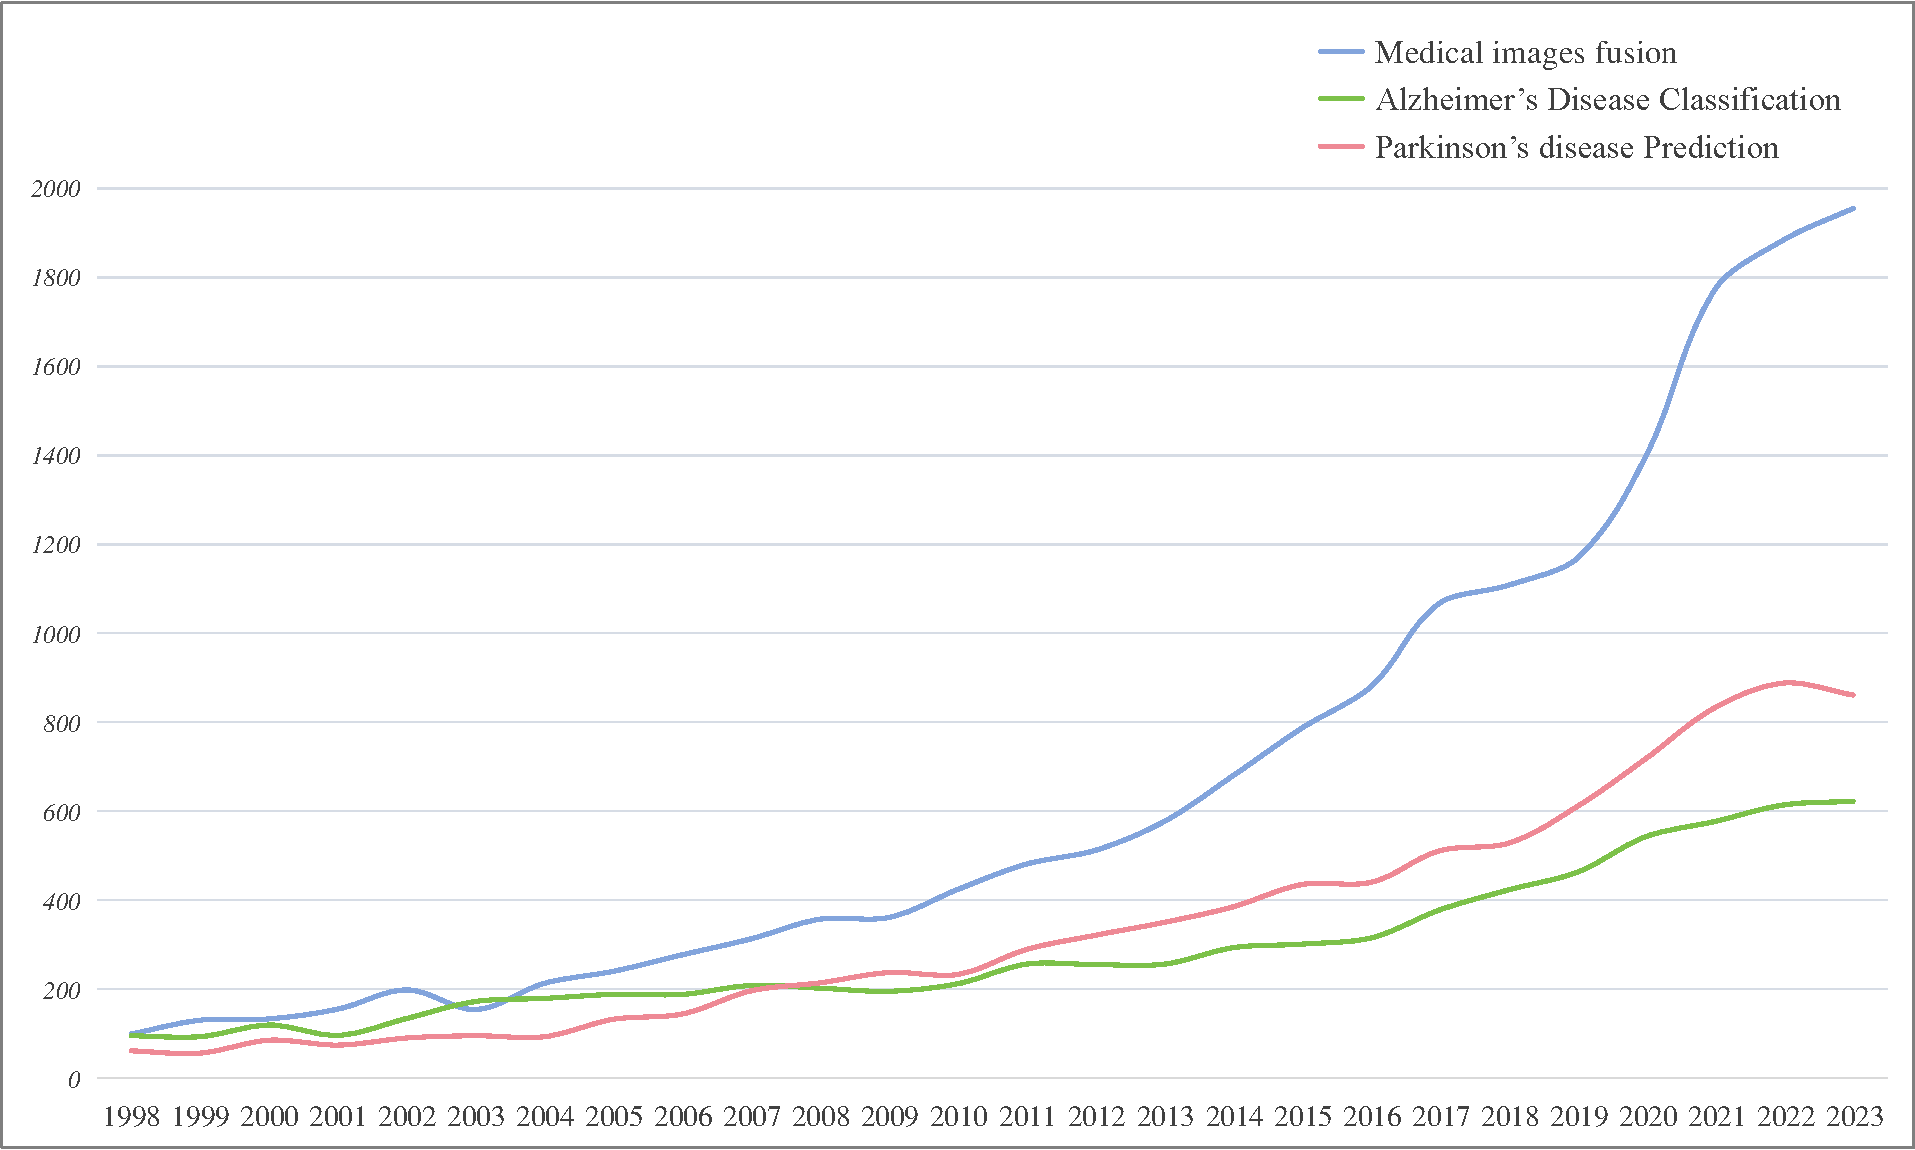
\includegraphics[width=0.9\linewidth]{figs/paperNumber.pdf}  
      \caption{按年搜索PubMed上三个关键词的发文量统计}\label{paperNumber}
    \end{figure}

基于智能辅助诊断的研究已经拓展至医学影像分析的多个领域,包括医学影像配准\cite{balakrishnan2019voxelmorph,ashburner2007fast}、医学影像分割\cite{sharma2010automated,zhou2018unet++,chen2021transunet}、医学影像融合\cite{anwar2018medical,dogra2023multi,tang2022image}、医学影像分类\cite{dai2021transmed,frid2018gan,wang2017chestx}、疾病检测\cite{gaitonde2017chronic,ferentinos2018deep}以及疾病预测\cite{dahiwade2019designing,shah2020heart,krishnamoorthi2022novel}等多个层面。将深度学习方法融入智能辅助诊断系统,
%不仅提高了诊断的准确性和效率,更为医学影像领域的发展注入了强大的活力,成为当前最具前景的技术路径之一。展望未来,随着技术的不断演进和深度学习算法的不断优化,我们有望目睹智能辅助诊断在医学领域发挥更为重要的作用。这
不仅将为医生提供更为准确、快速的诊断工具,也将为患者制定更加个性化和精确的治疗计划,推动医学影像技术不断走向新的高峰。
%因此,投身于深度学习方法在医学影像领域的研究与应用,将成为科技领域中最富有挑战性和前瞻性的研究方向之一。
本文将深入探讨多模态的医学影像融合、AD的影像分类及PD的疾病预测。图1.1统计了在PubMed上按年搜索“Medical images fusion”、“Alzheimer’s Disease Classification”以及“Parkinson’s disease Prediction”这几个关键词的文章数量,从中可以发现,在过去的25年里,基于智能辅助诊断的研究越来越受到关注。其中,多模态医学影像融合的研究正在以惊人的速度增长,其潜在的应用价值和社会影响不容小觑。

\subsection{多模态医学影像融合}
%随着影像处理技术的不断成熟和进步,影像融合技术正逐渐成为各个领域的研究热点,其中医学影像融合技术的崛起更是为医疗领域带来了全新的可能性。
在临床影像诊断中,医学影像融合技术能够将来自不同模态的医学影像(如CT、MRI、PET等)有效地融合,提供更全面、立体的信息,有助于医生更准确地诊断病变或异常情况。此外,医学影像融合还可以用于手术规划和导航,在手术过程中为医疗专业人员提供即时且高清的影像资料,旨在提升外科手术的精确性及保障患者的安全。在当前的研究中,医学影像融合算法主要分为基于传统方法和基于深度学习方法两大类别。


\subsubsection{基于传统理论的融合方法}
传统的医学影像融合方法涵盖了多种算法,其中包括基于稀疏表示\cite{liu2015general,maqsood2020multi,li2021medical}、基于形态学\cite{matsopoulos1994multiresolution,mukhopadhyay2001fusion,liu2019medical}、基于模糊理论\cite{ali2015multi,hu2021fuzzy,velmurugan2018multimodality}、基于多尺度分解\cite{jin2016medical,li2017pixel,singh2014fusion,yin2018medical}及基于机器学习的融合算法\cite{jasti2022computational,raja2020artificial,alseelawi2022novel,tang2019augmentation,diwakar2021latest}。
这些方法各自在不同场景下都表现出一定的优势,基于多尺度分解的融合方法由于其能够在不同尺度层面上进行信息处理,因而引起了广泛的研究兴趣。多尺度分解技术将影像转化为具有分层结构的多个尺度表示。这种分层结构的设计能在评估时兼顾影像的整体特性和具体细节,进而实现对影像深层意义的更全面理解。通过将影像分解成不同分辨率的子影像,多尺度分解允许独立处理不同层次的影像信息,有效地促进了对影像中关键特征的提取。这样的方法不仅有助于全局与局部信息的融合,还为影像处理提供了一种更为灵活、全面的手段,以适应不同尺度下的影像结构。基于多尺度分解的融合方法具备明显优势,能有效保留影像细节、融合全局与局部信息,同时增强特征表示,为影像处理任务提供强大支持。

拉普拉斯金字塔是典型的多尺度方法,特征金字塔的核心理念在于通过构建多尺度的影像表示,有助于系统更全面地理解影像中的对象特征,从而提升物体检测和识别的性能。Wang等人\cite{wang2011multi}将拉普拉斯金字塔变换的原理作为影像融合策略,该方法主要包括三个步骤
%,如图\ref{Pyramidfusion} 所示
。首先,分别对每个源影像进行拉普拉斯金字塔分解,然后采用不同的融合规则对新的每个拉普拉斯金字塔级别进行融合。对于最顶层,采用最大区域信息规则;对于其余级别,采用最大区域能量规则。最后,通过反向拉普拉斯金字塔变换得到融合影像。使用两组影像验证了提出的融合方法,并与其他融合方法进行比较。通过分析实验结果的分析显示,这种方法表现出了较好的性能,融合影像的质量优于其他方法的结果。
在医学影像融合领域,基于多尺度分解的方法通过将医学影像分解为不同尺度的子影像,分别进行处理并最终融合,以确保在整个处理过程中更好地保留影像的结构和细节信息。这种策略使得医生在进行临床诊断时能够获得更全面的信息,从而提高了对患者病情的准确评估。多尺度分解的融合方法在医学影像处理中的引入,强调了在融合过程中对影像多层次特征的关注,这种思想的实际应用在\cite{sahu2014medical,mi2021medical,jiang2023lightweight}等文章中大放异彩。
 \if 0
   \begin{figure*}[htbp]
      \centering
      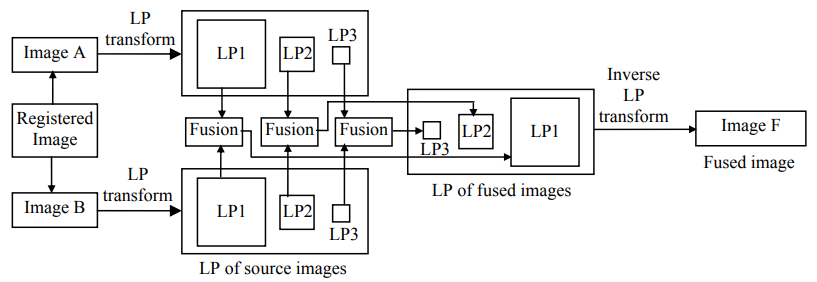
\includegraphics[width=0.95\linewidth]{figs/LaplacianPyramid.png}
      \caption{基于拉普拉斯变换的融合方法框架}\label{Pyramidfusion}
    \end{figure*}
  \fi

传统的融合方法中,医学影像融合通常依赖于人工设计的特征和规则,通过影像处理技术实现对不同模态医学影像的融合。这种方法在早期为医学影像的综合分析提供了基础,但受限于人工设计的特征和规则,其应用范围和效果逐渐受到限制。

\subsubsection{基于深度学习的融合方法}
近年来,随着深度学习技术的迅速发展,基于深度学习方法的医学影像融合技术\cite{rajalingam2018multimodal,liu2018deep,kaur2021multi,xia2019novel,zhou2023deep,rajalingam2022intelligent}取得了显著的突破。深度学习模型,特别是卷积神经网络(CNN)\cite{wang2020multi,el2021efficient,xia2019novel,li2021novel,zhang2023medical}以及生成对抗网络(GAN)\cite{zhou2023gan,huang2020mgmdcgan,ma2020ddcgan,wang2021dicyc}等,能够自动学习影像中的复杂特征和模式,从而实现对医学影像的更精细、准确的融合。这使得医学影像融合技术在影像诊断、手术导航等领域发挥着越来越重要的作用。

Lahoud等人\cite{lahoud2019zero}利用预训练神经网络,通过提取深度特征图进行影像融合,实现将来自多模态源影像的信息整合到单一输出中。与传统方法不同,该方法采用了新颖的策略,通过比较特征图生成融合权重,推动多模态影像的融合过程。这一方法不仅适用于两幅影像的融合,还可以扩展到任意数量的输入来源。实验证明,该技术在视觉质量、客观评估和运行效率方面均有较好的效果。Kaur等人\cite{kaur2021multi}提出了一种采用多目标优化策略结合深度学习的医学成像处理方法,实现了不同模态的医学影像之间的有效整合
%,如图\ref{fusionDL}所示
。该方法首先使用非子采样轮廓波变换(NSCT)将影像分解为子带。随后,采用Inception的极端版本(Xception)对源影像进行特征提取。使用多目标差分演化算法进行特征优化。之后,通过决定系数和一种基于能量损耗的融合策略来计算融合权重。最后,借助逆非子采样卷积变换构建融合后的影像。根据实验数据,这种方法在多模态影像融合技术中显示出明显的优势。
  \if 0
   \begin{figure*}[htbp]
      \centering
      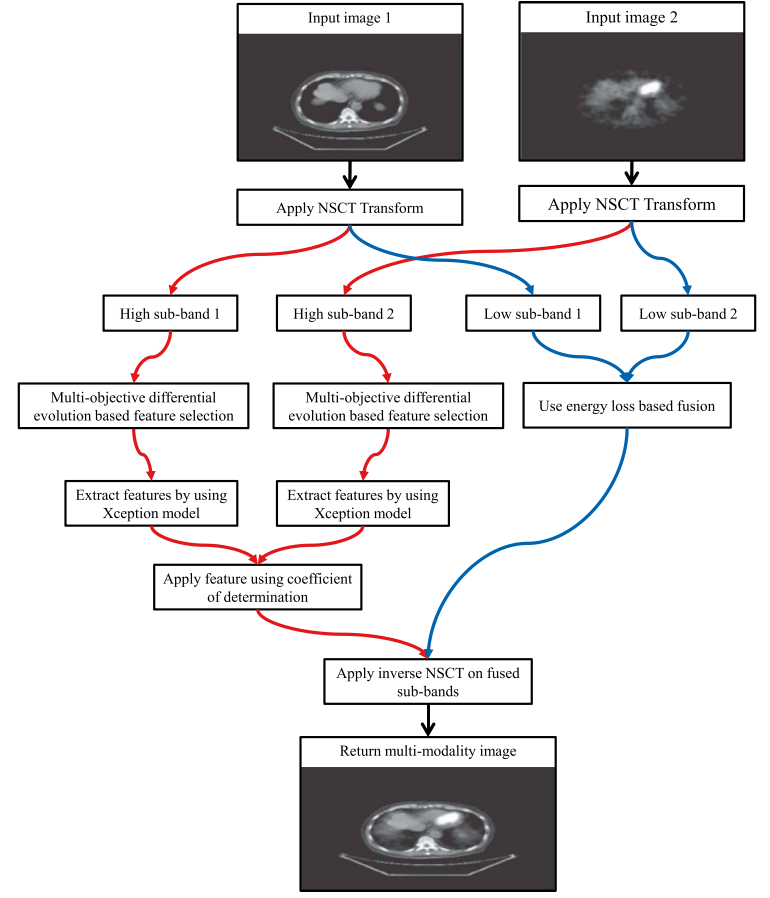
\includegraphics[width=0.95\linewidth]{figs/fusionDL.png}
      \caption{基于多目标差分进化的深度神经网络的多模态医学影像融合}\label{fusionDL}
    \end{figure*}
  \fi
  
Zhou等人\cite{zhou2023gan}总结了生成对抗网络(GAN)在深度生成模型领域的研究热点,特别是在医学影像融合方面的广泛应用。首先,从基本模型和训练过程两个方面阐述了GAN的基本原理;其次,将变种GAN模型总结为三个方向(概率分布距离、整体网络架构、神经网络结构),从基于f-散度的方法、基于IPM的方法、单生成器和双鉴别器GAN、多生成器和单鉴别器GAN、多生成器和多鉴别器GAN、条件约束GAN、卷积神经网络结构GAN和自动编码器神经网络结构GAN等八个维度总结了近年来的典型模型;第三,从三个方面探讨了GAN模型在医学影像融合领域的优势和应用;第四,介绍了GAN面临的主要挑战以及在医学影像融合领域所面临的挑战。
Ma等人\cite{ma2020ddcgan}介绍了一种带有双重鉴别器的条件式生成对抗网络(DDcGAN)框架,专门用于整合具有不同清晰度的红外与可见光图像。此模型利用生成器和两个鉴别器之间的对抗性互动机制,实现了在融合影像中同时保留红外影像的热辐射和可见影像的纹理细节。为了融合不同分辨率的源影像,DDcGAN采用降采样策略,以确保融合影像在保持信息清晰度的同时避免热辐射或纹理细节的丢失。该方法不仅在红外和可见光影像融合上表现出色,还在融合多模态医学影像方面取得了卓越的结果。

基于深度学习的医学影像融合不仅能够提高影像的清晰度和对比度,还能有效地在处理过程中维持影像的重要细节和内容,为医生提供更全面的诊断依据。此外,这些技术还有助于将不同模态影像之间的信息关联起来,为综合性医学分析提供更准确的数据支持。

\subsection{阿尔茨海默症的分类}
AD作为老龄化人群中常见的慢性神经系统退行性疾病,其主要特征表现为认知障碍和记忆缺失。由于其发病机制缓慢且目前难以完全治愈,早期发现和区分中度认知功能障碍(Mild Cognitive Impairment,MCI)和AD对于实施有效的干预和治疗至关重要。值得注意的是,MCI还分为两个亚型,即早期轻度认知功能障碍(Early MCI,EMCI)和晚期轻度认知功能障碍(Late MCI,LMCI),它们分别表示在认知功能下降中的不同阶段,EMCI通常早于LMCI发生。这样的细致划分对于更准确的病程分析和制定干预方案至关重要。然而,AD的影像诊断面临一系列挑战,因为实现精确分类依赖于能够明显区分不同类别的特征。诊断主要依赖于对患者脑部扫描影像的分析,涉及解决一个目标分类问题。由于脑部影像的微小差异和结构变化幅度相对较小,特征不够明显,如图\ref{fineAD},因此正确分类和判断阿尔茨海默症的病程变化具有较大难度。当前研究中,针对AD的影像分类算法主要分为两大类别:粗粒度分类(AD、NC和MCI这这种类别的2分类或者是3分类)和细粒度分类(早期分类,主要是将MCI细分成了EMCI好LMCI,再与AD或NC进行组合分类)。粗粒度分类主要关注整体疾病状态,而细粒度分类更注重对不同亚型的精准辨别。AD分类算法的发展旨在提高对MCI和AD的早期检测,以实现及时的干预和治疗,更好地预防或延缓疾病的进展。

   \begin{figure*}[htbp]
      \centering
      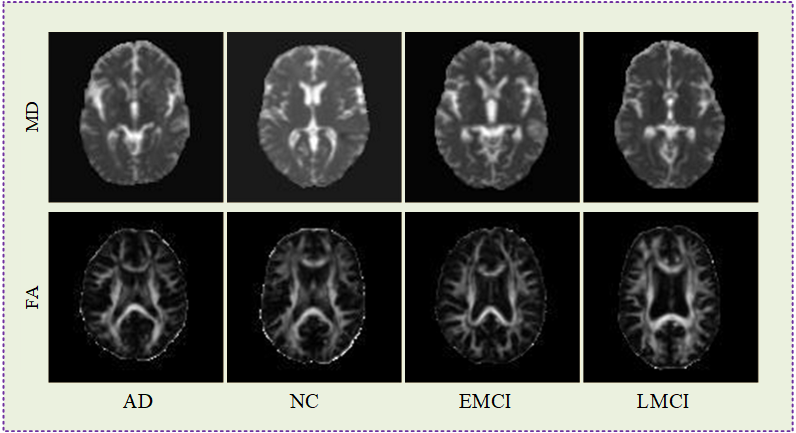
\includegraphics[width=0.9\linewidth]{figs/fineAD.png}
      \caption{四类(AD、 NC、EMCI、LMCI)受试者的两种DTI(弥散张量成像的分数各向异性(FA)和平均弥散率(MD))脑部影像}\label{fineAD}
    \end{figure*}
    
\subsubsection{基于粗粒度影像的分类应用}
本文探讨的问题是如何在AD、MCI以及正常对照组(Normal Control, NC)之间进行有效的分类。一些学者侧重于从脑部医学影像中抽取特定的AD病理特征进行分类\cite{gray2012multi,garali2015region,feng2021extracting,gray2011regional},例如海马、杏仁核及前额叶等关键脑区。Garali等人\cite{garali2015region}提出了一种新颖的方法,用于评估大脑区域在区分AD和健康脑影像方面的有效性。首先,将脑扫描数据分割并对齐至116个特定的解剖结构区域。然后计算这些区域的前四个时刻和直方图的熵。接着,使用接收器操作特性曲线对各个区域分离PET脑影像的能力进行排名。选取了21个区域作为输入,分别输入到支持向量机和随机森林分类器中,评估结果基于142个脑PET影像进行。分类结果较使用最初的116个区域或输入整个脑体素时更好。Feng等人\cite{feng2021extracting}提出了一种基于ROI的小波子带能量(ROICSE)特征方法,以在频域中表示sMRI影像进行AD分类。具体而言,sMRI扫描经过预处理步骤后,会使用预先定义的脑部掩膜进行分割,从而得到90个特定的兴趣区域(ROI)。与传统方法在空间维度上直接提取这些ROI特征不同,这里采用的是小波变换技术,对每一个ROI进行分析,从而获得其能量分布的不同子带。然后,对于一个ROI,构造一个子带能量(SE)特征向量来捕捉其能量分布和轮廓信息。随后,将90个ROI的SE特征向量串联起来形成sMRI影像的ROICSE特征。最后,使用支持向量机(SVM)将880名受试者的数据进行了分类,这些数据来源于ADNI和OASIS数据库。实验结果表明,AD vs. NC、MCI vs. NC和AD vs.MCI的准确率分别是93.57\%、83.13\%和82.73\%,ROICSE方法优于其他六种最先进的方法。Gray等研究者\cite{gray2011regional}将每位参与者的脑部MRI扫描细致地分割为83个不同的解剖部分。随后,他们使用这些解剖区域作为参考框架,从同个人的FDG-PET扫描中提取了各ROI的平均放射性标记强度数据。最终,通过分析这些强度值作为特征,利用SVM算法对样本进行了分类处理。在AD患者和NC对照组之间取得了出色的区分度(准确率82\%),在MCI患者和NC对照组之间取得了良好的区分度(准确率70\%)。
    \if 0
   \begin{figure*}[htbp]
      \centering
      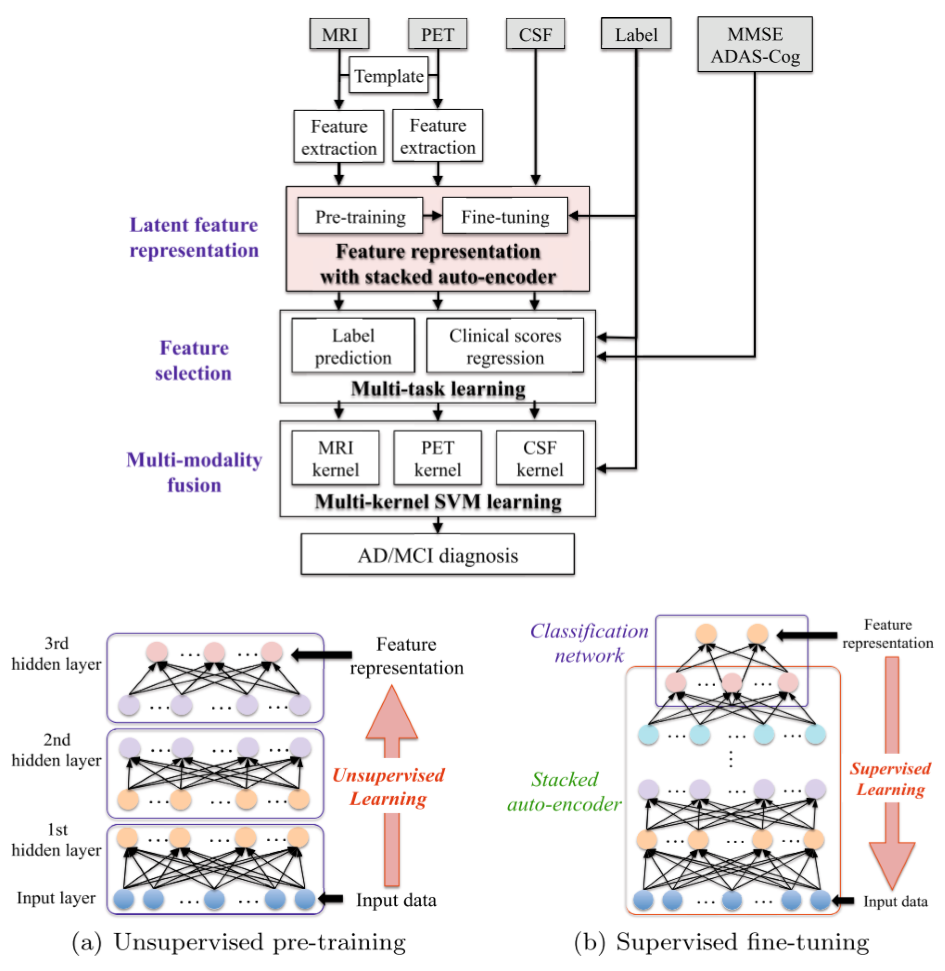
\includegraphics[width=0.95\linewidth]{figs/2classify.png}
      \caption{用于阿尔茨海默病的AD与MCI诊断的网络模型,潜在特征表示主要由堆叠自编码器(a)和两步参数优化方案(b)组成}\label{coarse2classify}
    \end{figure*}
    \fi
    
尽管基于特定区域的兴趣点的方法来提取关键特征并对这些特征进行深入分析的策略在某些方面表现出效力,但也存在一些明显的限制。首先,特征提取过程可能会受到人为因素的影响,导致错误,同时分析手段也可能存在局限性。由于AD标志物不明确,因此在划分和选择ROI时可能发生疏漏,极大地影响AD诊断的效果。再者,采用基于ROI的技术在实现时,模型训练通常需要依赖大规模的实验数据来保证预测结果的精确度,这无疑会增加显著的时间和人力资源消耗。而在阿尔茨海默病分类研究的现状下,采用ROI方法的研究者们普遍采取了多样化的影像预处理手段,包括但不限于影像与参考模板的精确对位、应用刚性或非刚性变换来适配不同的参照框架,以及对影像进行详细的区域分割处理。面对这些挑战,深度学习方法在AD影像分析中展现出卓越的潜力\cite{suk2013deep,so2019deep,suk2014hierarchical,tufail2021classification,khvostikov20183d}。深度学习通过学习数据中的特征,自动发现并表征影像中的复杂模式,避免了手动提取特征的繁琐过程。这使得深度学习在处理AD影像分类任务时更具优势。其对大规模数据的高效处理能力,以及在学习表征方面的卓越性能,使得深度学习方法成为应对上述问题的有力工具。

Suk等人\cite{suk2013deep}提出了基于深度学习的堆叠自编码器的特征表示方法
%,如图\ref{coarse2classify}所示
。为了创建一个可靠的AD/MCI分类模型,作者综合考虑了深层信息和基础特征,以此提高模型的诊断性能。实验证明,所提出的方法对于AD、MCI的诊断分别具有95.9\%、85.0\%的准确率。通过对训练模型的可视化观察,一种利用深度学习技术来获取神经影像数据中高级共享潜在特征的新方法被提出\cite{suk2014hierarchical}。具体而言,该框架以受限的玻尔兹曼机(DBM)为单元,能够从三维图像片段中识别并提取层次化的潜在特征。接着,应用多模态DBM对MRI和PET图像的对应区块进行了联合特征提取。为了评估所提出的方法的效能,进行了一系列详尽的实验测试,并与最先进的方法进行了比较。在AD vs. NC、MCI vs. NC分类问题中,分别获得了95.35\%、85.67\%的最大准确率,优于竞争方法。
So等人\cite{so2019deep}提出了一种结合纹理分析与深度学习的AD粗粒度分类方法。首先对MRI影像应用了三维灰度共生矩阵(GLCM)方法进行纹理分析。然后,使用Fisher系数选择适用于分类的特征。最后,利用多层感知器(MLP)模型将其分为AD vs. MCI、AD vs. NC和MCI vs. NC三类。该模型在分类准确性上表现出色,分别为AD vs. MCI(72.5\%)、AD vs. NC(85\%)和MCI vs. NC(75\%),并在混淆矩阵、支持向量机(SVM)和K最近邻(KNN)分类器的评估中展现出优越性。所提出的方法相较于SVM和KNN分类器至少提高了6-19\%的准确率。自动化的AD分类系统可以作为辅助工具,帮助医务人员诊断阿尔茨海默病的阶段,从而提供适当的医疗治疗。 
Khvostikov等人\cite{khvostikov20183d}提出了一种基于3D Inception的卷积神经网络(CNN)的设计,用于AD的诊断。该网络注重内部资源的利用,通过在海马ROI上融合sMRI和DTI模态。与传统的基于AlexNet的网络相比,表现显著更好。AD vs. MCI vs. NC、AD vs. NC、AD vs. MCI与MCI vs. NC这些分类的准确率分别是68.9\%、93.3\%、86.7\%和73.3\%。

%从脑部医学影像中抽取特定的AD病理特征诊断的方法相对基于深度学习诊断的方法精确度略低。但,关于AD的粗粒度分类问题主要包括二分类(AD vs. NC、AD vs. MCI和MCI vs. NC)或三分类(AD vs. MCI vs. NC),无法辅助诊断更进一步的多阶段。
尽管在脑部医学影像中提取特定的AD病理特征的方法在精确定位疾病迹象方面取得了一定的成果,然而,与那些依赖深度学习的诊断技术相比,这些传统方法在精确度上稍显不足。这可能是因为这些传统方法主要关注单一或少数感兴趣区域(ROI),而对于复杂的神经影像数据,这种精细的特定特征提取方式难以涵盖疾病的整体情况。
特别是在处理AD的粗粒度分类问题时,通常涉及二分类(AD vs. NC、AD vs. MCI和MCI vs. NC)或三分类(AD vs. MCI vs. NC)的任务。这些任务主要旨在初步判别患者的整体状态,而未能提供关于疾病进展更详细信息的细致分析。相比之下,基于深度学习的方法通过学习大量数据中的特征,具有更强大的表示学习能力,可以更全面地捕捉疾病的复杂模式和变化。
这种方法的优势在于其对大规模和多模态数据的高效处理,以及对于特征学习的自动化处理。这种自动化处理避免了手动提取特征时可能引入的主观性和繁琐性。因此,基于深度学习的方法展现出更高的潜力,有望推动AD诊断领域向更为准确和全面的方向发展。这不仅提供了更有力的支持,还有助于更全面地理解和干预AD等神经系统疾病的发展过程。
    
\subsubsection{基于细粒度影像的分类应用} 
尽管AD的粗粒度分类方法在筛查、早期检测和初步诊断方面具有一定的实用性,对于医务人员而言,在多阶段AD的诊断中进一步了解疾病的不同阶段、进展速度以及相关病理学变化,对个体化的治疗方案和干预手段更具有指导意义。目前,关于AD的智能辅助诊断的研究在多个AD进行性阶段方面的适用性相对较少。近年来,越来越多的学者对AD进行了细粒度的研究,例如\cite{korolev2017residual,ruiz20203d,song2019graph,parmar2020spatiotemporal,pan2020early,basaia2019automated,helaly2021deep,fu2021automated,shamrat2023alzheimernet}等。

Korolev等人\cite{korolev2017residual}采用残差网络和普通3D卷积神经网络结构,应用于3D结构性MRI脑扫描的AD与MCI以及NC的分类任务中,涉及到AD与NC、EMCI、LMCI之间的多类别分类。该研究展现了在细粒度分类上的一定成果,不仅涉及AD vs. NC,还包括了AD vs. EMCI、AD vs. LMCI、LMCI vs. NC等任务,其结果表明了模型在处理这些复杂分类问题上的鲁棒性。实验测试的准确率分别是:AD vs. NC: 80\%,AD vs. EMCI: 63\%,AD vs. LMCI: 59\%,LMCI vs. NC: 61\%,LMCI vs. EMCI: 52\%,EMCI vs. NC: 56\%。
Ruiz等人\cite{ruiz20203d}则提出了一种集成方法,采用3D密集连接卷积网络(3D DenseNets)模型进行四分类,即AD、EMCI、LMCI和NC。这种方法通过密集连接改善模型内部数据的流动,同时采用概率融合方法合并每个独立分类器模型的概率输出。在测试中,该方法相对于处理3D MRI的其他最新方法表现更好,获得了66.67\%的准确率,为细粒度分类提供了可行的解决方案。
    
Song等人\cite{song2019graph}使用图卷积神经网络(GCN)进行网络分类,将受试者分为NC、EMCI、LMCI和AD四个类别,实现了89\%的准确率。Parmar等人\cite{parmar2020spatiotemporal}通过使用经过修改的3D卷积神经网络设计了一种简化而准确的方法,从静息状态fMRI数据中提取特征并对AD进行四分类。该研究中的CNN设计保留了更多的空间和时间信息,获得了93\%的准确率,为对AD进行多阶段诊断提供了一种潜在的有效途径。
Helaly等人\cite{helaly2021deep}则采用两种基于深度学习的方法对医学影像进行AD四个阶段(AD vs. EMCI vs. LMCI vs. NC)的分类。这两种方法分别基于简单的CNN架构和迁移学习原理,使用不同的模型进行医学影像分类。具体来说,第一种方法使用简单的CNN架构,该架构基于2D和3D卷积处理数据集为2D和3D的脑部扫描。第二种方法应用迁移学习原理,利用预训练的模型(VGG19模型)进行医学影像分类。这两种方法分别取得了93.61\%和95.17\%的准确率,为多阶段AD分类提供了更多选择。
 \if 0
   \begin{figure*}[htbp]
      \centering
      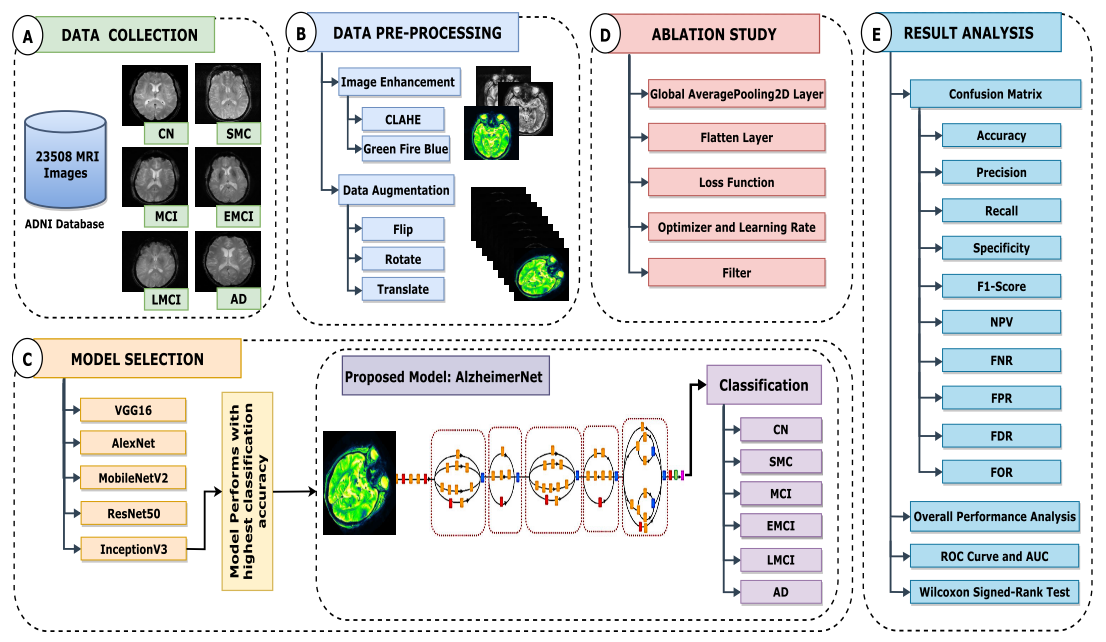
\includegraphics[width=0.95\linewidth]{figs/5classify.png}
      \caption{用于阿尔茨海默病的多分类(SMC、AD、NC、MCI、EMCI、LMCI)的网络模型(AlzheimerNet)结构}\label{fine5classify}
    \end{figure*}
 \fi
 
少数研究还对AD的进行性阶段(包括NC、主观记忆问题(SMC)、EMCI、MCI、LMCI和AD)进行了多类别分类\cite{shamrat2023alzheimernet,ramzan2020deep},进一步拓展了对AD多阶段的认知。Shamrat等人\cite{shamrat2023alzheimernet}提出的AlzheimerNet分类器具有更细致的多阶段诊断能力
%,分类器结构如图\ref{fine5classify}所示
。通过精细调整的卷积神经网络(CNN)架构,该模型可以识别阿尔茨海默病的五个阶段,包括SMC、MCI、EMCI、LMCI和AD以及NC类别。在六分类任务上,通过比较五个预训练模型(VGG16、MobileNetV2、AlexNet、ResNet50和InceptionV3)和AlzheimerNet模型在各种性能指标上的表现,该模型表现出98.68\%的准确率,显示出了在多阶段AD诊断中的出色性能。

在AD的细粒度分类方法中,主要集中在二分类任务,例如AD与EMCI、AD与LMCI、LMCI与NC、LMCI与EMCI等。这些二分类任务在当前研究中占据主导地位,主要受到深度学习方法的广泛运用。就二分类而言,研究结果表明,这些方法在AD的早期诊断、疾病阶段划分以及患者与正常对照的区分等方面取得了显著的成果。例如,Korolev等人\cite{korolev2017residual}在AD vs. NC、AD vs. EMCI、AD vs. LMCI等任务中实现了可观的分类准确性,为早期AD的精准辨别提供了可能性。相比之下,三分类任务(如AD vs. EMCI vs. LMCI、NC vs. EMCI vs. LMCI)相对较少,研究涉及更多的类别,需要更高的分类难度和挑战。在这方面,尚未形成广泛的研究共识。

然而,一些初步的研究显示,在处理多类别分类问题时,模型的性能仍然具有潜在的优势。通过更全面的分类,有望提供更丰富的信息,为医务人员提供更全面的诊断参考。
六分类任务,涉及到NC、SMC、EMCI、MCI、LMCI和AD的分类,是相对较少见的研究方向。在这一领域,Shamrat等人\cite{shamrat2023alzheimernet}提出的AlzheimerNet分类器在实现六分类任务上表现出色,具有98.68\%的准确率,显示了对多阶段AD进行细致分类的强大潜力。这种细粒度的多分类方法有望为医疗决策提供更详细的信息,推动个体化治疗和干预的发展。
绝大多数采用深度学习方法的AD细粒度分类方法,其准确率存在一定的差异,取决于模型的架构设计、数据集质量以及训练过程中的参数调整等因素。在这方面,不同的研究方法可能呈现出高低不一的性能。然而,总体趋势显示出深度学习方法在解决AD细粒度分类问题上的潜在优势,通过学习丰富的影像特征,更全面地捕捉疾病的多样性,为提高AD诊断的准确性和全面性提供了有效途径。


\subsection{帕金森疾病的预测}
帕金森症(PD)是一种长期性的神经退行性疾病,它直接作用于那些在大脑中制造多巴胺的关键神经元。这种疾病在神经系统疾病中的发病率排在第二位,仅次于AD\cite{prusiner2001neurodegenerative,leroy1998deletions}。
许多患有PD的患者在被诊断时已处于病情的中到晚期阶段,这使得他们失去了接受最佳治疗的理想时机。\cite{de2019prognosis,papagno2018cognitive}。因此,急需开发出更快捷、更精确、更具效能的检测技术,以便实现对PD的早期识别\cite{jyWen}。可作为PD预测的数据主要包括医学影像数据和临床数据。
医学影像数据可以呈现出脑部结构和活动的直观影像,有助于观察神经元损伤和多巴胺生成的变化。临床数据则提供了更全面的患者信息,包括症状描述、家族病史以及其他相关的临床特征,这些信息对于全面评估患者的健康状况至关重要。
将医学影像数据和临床数据相结合,可从多个角度来分析和理解帕金森病的发病机制,从而构建出更精确、更可靠的早期诊断模型。这样的模型不仅能提高诊断的准确性,还能为患者提供及时的治疗建议,提升生活品质并减缓病症进展。

\subsubsection{基于医学影像的预测方法}
在医学影像学领域,不断涌现新技术以助力帕金森病(PD)的诊断。这些技术因其独特的优势而备受瞩目,预计将大幅提升诊断的准确性。医学影像学提供了多种影像类型,如磁共振成像(MRI)揭示了大脑结构的细微差异;功能性磁共振成像(fMRI)捕捉了脑部活动模式;结构磁共振成像(sMRI)评估了大脑组织的形态改变;单光子发射计算机断层扫描(SPECT)和正电子发射断层成像(PET)则用于检测大脑代谢异常;弥散张量成像(DTI)描绘了神经纤维束的走向和完整性。这些技术共同为PD的早期发现与治疗提供了强有力的工具。


基于体素的形态测量学(voxel-based morphometry,VBM)技术利用MRI扫描快速且精确地量化脑部形态变化,如小脑的体积减少,并能在宏观层面迅速定位帕金森病(PD)的脑结构异常\cite{li2018patterns,de2017loss}。这项技术在成本效益和诊断准确性方面表现出色,已被临床研究所证实。Amoroso等学者\cite{amoroso2018complex}通过分析大脑肌肉萎缩与疾病严重度的关系,创建了一套全面的脑结构网络模型,其疾病分类准确度超过了94\%,优于标准VBM分析。另外,Rojas等人开发了一种基于SPECT影像的经验模式分解新技术\cite{rojas2013application},结合PCA提取关键特征并运用SVM进行分类,实现了高达95\%的准确率。Alexandra等人\cite{abos2017discriminating}通过对两组独立的受试者的静息态功能磁共振影像进行分析,并运用随机逻辑回归挑选特征输入SVM,在测试集中达到了80\%的预测准确率。

Francisco等研究者\cite{oliveira2018extraction}开发了一种新技术,通过分析FP-CIT SPECT影像来预测PD,并通过运用支持向量机(SVM)、K最近邻(KNN)以及逻辑回归这三种不同的机器学习模型,实现了97.9\%的高分类精度。此外,Martinez等人\cite{martinez2018convolutional}采用FP-CIT SPECT的医学影像数据结合CNN架构,包括LeNet3D与Alexnet3D,对PD进行了分类,其中Alexnet3D的分类准确度为94.1\%,曲线下面积为98.4\%。Kim等人\cite{kim2018artificial}应用了Inception V3网络进行PD预测,获得了87\%的曲线下面积。Castillo等人\cite{castillo2018robust}提出了一个集成学习的分类模型,结合了SPECT影像数据和多种生物学标记,构建了一个加权分类模型,该模型的分类准确度为96\%。这些研究成果显示,利用医学影像数据的PD预测技术正在持续改进,这些技术不仅提高了预测的准确性,还引入了多种先进技术和深度学习框架,为PD的早期诊断提供了更稳健和精确的工具。


\if 0
   \begin{figure*}[htbp]
      \centering
      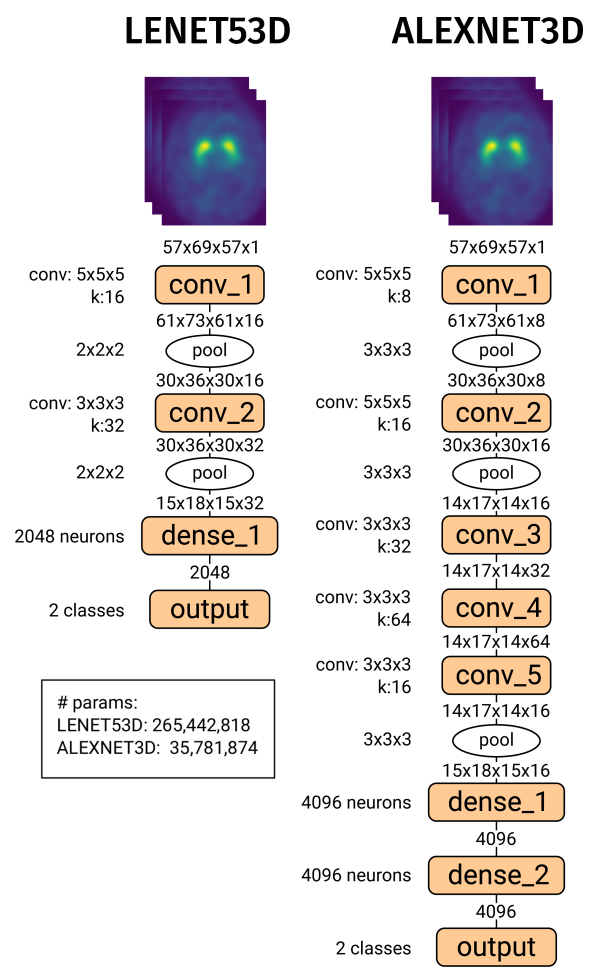
\includegraphics[width=0.8\linewidth]{figs/imagePredict.png}
      \caption{Lenet53D和Alexnet3D网络模型结构\cite{martinez2018convolutional}}\label{prePDimage}
    \end{figure*}
\fi    


近期研究通过DTI技术深入分析了患者的症状,进一步揭示了白质网络中神经元损伤的情况,并将其与正常对照组进行了比较。结果显示,PD和MCI患者的额叶白质网络功能损伤较为集中,且认知网络的全面功能失调和多个神经元认知网络在频率域内所表现出的功能损伤之间存在直接联系\cite{wang2020changes}。
多模态MRI数据融合了磁共振成像的特点与早期疾病检测的优势,为PD的早期发现提供了有价值的影像学生物标志物\cite{jyWen}。尽管sMRI和DTI单模态技术能够较好的反映血脑网络的宏观结构变化,但它们在功能形态层面上仍有不足。Rs-fMRI主要用于评估缺血性痴呆患者的脑灰质异常,但目前尚未能够全面且系统地评估其对脑白质异常所导致的神经元活动失常以及相关的脑功能变化和特征\cite{jyWen}。此外,针对大脑黑质皮层区域,现有的磁共振扫描成像技术也存在一定的局限性。尽管对该区域的异常表现具有较高的灵敏度,但在描述这些特征时仍然面临着复杂性、模糊性以及单一性的问题。

为了克服这些技术挑战,研究者们开始采用多模态检测和多重MRI异常检测技术,融合多种特征进行综合分析。该方法通过多角度、多层次地分析PD的神经病理状况,实现了对疾病的全面诊断及治疗效果的综合评价。它为中国PD神经病理学的临床诊断和评估提供了一个较为完善、成熟、合理且可靠的新途径\cite{pyatigorskaya2018comparative,gu2016automatic,bowman2016multimodal}。Pyatigorskaya等人\cite{pyatigorskaya2018comparative}首个遵循国际准则对NMS-MRI信号进行详尽剖析的工作,旨在揭示黑质中的质子体积与信号强度的特定特征,并在DTI技术支持下,分析了局部各向异性的特性及其信号组合模式。成功将PD的预测准确率提升至93\%。Bowman等人\cite{bowman2016multimodal}则采用融合的策略,并分析和讨论了rs-fMRI、sMRI以及DTI中的组织结构特性。
经综合考虑多种影像学指标如灰质密度、各向异性分数和功能连接等,以区分PD患者与正常对照组。通过这种多模态分析方法,他们达到了98.9\%的分类准确率,这一结果显著优于仅依赖单一影像模态的传统方法。这些发现不仅增强了对PD神经生物学特征的理解,而且为临床上PD的早期识别和治疗策略的制定提供了重要的影像学参考。

在医学影像领域,针对PD的早期诊断技术正在不断进步,涵盖了包括sMRI、扩散张量成像(DTI)和静息态功能磁共振成像(rs-fMRI)在内的多种成像手段。这些技术能够揭示出具有高度特异性的影像学生物标志物,从而增强了对PD早期阶段的识别能力。尽管如此,每种技术也面临着自身的挑战;例如,sMRI和DTI在捕捉功能性形态变化方面存在不足,而Rs-fMRI在评估脑白质皮层异常的神经元变化时则可能受到限制。为了克服这些限制,研究者们开始探索多模态检测和多重MRI异常检测技术的应用。这种方法通过综合不同MRI技术的优势,从多个维度和视角对PD进行全面的临床诊断和疗效评估。现有的研究\cite{pyatigorskaya2018comparative,gu2016automatic,bowman2016multimodal}表明,这种多模态方法能够取得较高的预测准确性,为我国在PD神经病理学临床诊断评估指标方面提供了新的思路和方法。


\subsubsection{基于临床数据的预测方法}
医学领域的临床资料丰富且多元,为深入研究PD提供了宝贵资源。临床资料广泛涉及病患的生理和生化指标,其中蕴藏着揭示PD特征的关键信息,对于预测PD的发展趋势具有重要价值。基于这些临床数据的PD预测方法,对于指导医学实践和治疗方案的制定具有重要意义。

在认知障碍领域,PD患者常伴有帕金森病痴呆(Parkinson’s disease dementia,PDD),及时识别其进展对患者的治疗和生活质量具有重大影响。为此,Kim等人\cite{kim2019prediction}采用了三种常用的认知评估测评——蒙特利尔认知评估(MoCA)、马蒂斯痴呆分级量表(DRS-2)和简易的精神状态测评表(MMSE),并使用回归模型评估了它们在预测PD认知进展方面的效能。研究发现,在条件一致情况下,MoCA在诊断PD轻度认知障碍(PD-MCI)和PDD方面的准确性最高,分别达到了AUC=0.79和AUC=0.89,敏感性分别为76.4\%和81.0\%。这一成果首次证明了MoCA可以作为预测PDD发生的指标。尽管MoCA在检测和预测PD-MCI和PDD进展方面获得了较好的应用\cite{hu2014predictors,pigott2015longitudinal,marras2013measuring,hoops2009validity,dalrymple2010moca},但MoCA的低特异性限制了它作为诊断工具的实用性\cite{marras2013measuring,hoops2009validity},这反映了PD进展的复杂性以及当前缺乏可靠的客观生物标志物\cite{miller2015biomarkers}。因此,开发更先进的PD进展预测模型或更精确的诊断策略,对于选择合适的临床试验参与者显得尤为重要。

随着海量数据集的涌现,特别是那些涵盖纵向研究和多维度信息的数据集\cite{latourelle2017large,simuni2016predictors,holford2006disease},为PD进展预测模型的构建迎来了新的发展契机。例如,Diba等研究者\cite{ahmadi2019parkinson}通过机器学习技术分析PD的血清样本的研究,揭示了外周炎症标志物与PD症状间的联系。研究结果表明,患者初始阶段的外周炎症水平对于预测其病情的未来演变具有重要意义。Chan等人\cite{chan2007levodopa}提出的预测模型,证实了诸如左旋多巴之类的药物在控制PD发展和改善患者症状方面的显著疗效。
也有学者利用生物力学测量,包括步态和姿态的平衡能力,构建了预测PD患者两年之内进展的网络模型\cite{raval2020prediction},该模型采用CNN技术预测MDS-UPDRS第三部分评分的两年变化率,为针对快速进展型PD的药物治疗提供了新思路。
另外,Latourelle等人\cite{latourelle2017large}的研究指出,临床基线的运动评分数据是预测PD未来发展速度的关键因素之一。

在PD的初期阶段,及时检测非运动症状对于控制病情发展极为重要。Nilshi及其同事\cite{nilashi2020remote}开发了一种新的远程监控PD进展的技术,该技术融合了深度学习与聚类分析两种方法。具体实施时,研究团队采用了深度信念网络(DBN)结合支持向量回归(SVR)的策略来预测PD的UPDRS评分,并构建了多个时间尺度上的DBN预测模型。为了提升预测的性能,研究中还引入了自组织映射(SOM)的聚类技术,并通过SVR对DBN模型的预测结果进行整合优化。研究成果表明,这种结合聚类与DBN,再通过SVR进行结果融合的方法,在预测Total-UPDRS和Motor-UPDRS方面均优于单一的SOM、DBN或SVR技术。具体而言,在预测Total-UPDRS时,测试集上的均方根误差(RMSE)与决定系数(R2)分别达到了50.8\%与93.3\%;在预测Motor-UPDRS得分方面,模型的均方根误差(RMSE)为52.1\%,决定系数(R2)则达到91.4\%。这一技术开辟了远程监控PD患者病情进展的新途径。

在医学研究领域,对PD的多样化临床数据进行深入分析,是揭示疾病预测因素的关键。当前研究重点之一是对比不同的认知评估测试,其中蒙特利尔认知评估(MoCA)在检测PD认知障碍方面显示出较强的能力,尽管如此,其低特异性问题仍待克服。结合大型数据集及ML技术,PD的进展预测模型得到了显著提升,特别是在生物标志物和基因与疾病关联的探索上。总体来看,PD的研究正步入充满希望的新阶段,为更有效的疾病干预和治疗策略提供了坚实的科学支撑。

    
\section{本文的主要工作}
本项研究聚焦于智能辅助影像组学分析技术在医学辅助诊断领域中的应用,特别关注脑肿瘤、AD和PD。关键技术手段涵盖影像融合、影像分类与疾病预测。本文的主要工作包括:
\begin{itemize}
    \item 在多模态医学影像融合方面,本文分析了MRI、CT、PET、SPECT及其他医学影像,归纳总结了其各自隐藏的医学语义信息,并与影像特性对应,设计了一个医学语义引导的双分支网络。另外,本文从多个维度如低频、高频和多尺度出发,分析不同的空间、通道特征,提出三种特征提取模块。并结合自适应线性融合策略,提出一种多模态脑影像融合的网络模型。这两种方法都得到了临床医师较高的评价。
    \item 在AD诊断方面的研究上发现了AD不止有三类(AD、NC和MCI),其中MCI还可以分期,细分为EMCI和LMCI。EMCI阶段是可逆的,及时发现和干预可以避免AD的发展,而在LMCI阶段及时诊断和治疗可以延缓AD的发展或治愈AD。另外,由于绝大多数基于深度学习方法的应用都难于获得全局的特征,而频域的处理可以做到。因此,本文提出了一种小波卷积单元,并将其应用于AD的细粒度多分类。
    \item 在PD诊断领域,本文归纳总结了现阶段国内外学者在PD预测上的研究工作,将其定义为静态和动态预测两种类型。针对当前的研究现状,本文讨论和分析了PD智能诊断未来的研究趋势。另外,本文在PD基线的跨模态(除了考虑影像层面的数据外,还结合了非影像类数据)数据中,筛选了代表PD进展的关键特征。其次将跨模态的数据融合,应用于PD的进展预测,并提出了一种跨模态融合预测进展的方法,有利于临床预测性能的提升。
\end{itemize}


本研究课题内的各工作环节间存在着紧密的相互联系与支撑。首先,通过引入首个关于多模态医学影像融合的任务,确立了医学语义的核心概念,这一理念继而被融入第二个融合方法中,显著增强了影像的可解释性,为病灶的精确定位与动态追踪提供了有力支持。在实施这两项多模态融合技术的同时,现有神经网络模型在捕获全局特征方面的局限性被意识到,进而促成了第三个工作——即通过优化网络结构以有效拓展感受野,并成功应用于AD的细粒度分类,实现了诊断精度的新突破。
进一步地,本文巧妙地将多模态影像融合的思路迁移至跨模态数据融合的领域,特别是在帕金森病(PD)病情进展预测的研究中,这一思路的应用极大提高了预测的准确性。综上所述,这些工作的依次开展不仅在技术层面上形成了层层递进的创新链,还拓宽了技术应用范围,共同促进了智能辅助影像组学技术的发展与临床价值提升。


   \begin{figure}[ht]
      \centering  
      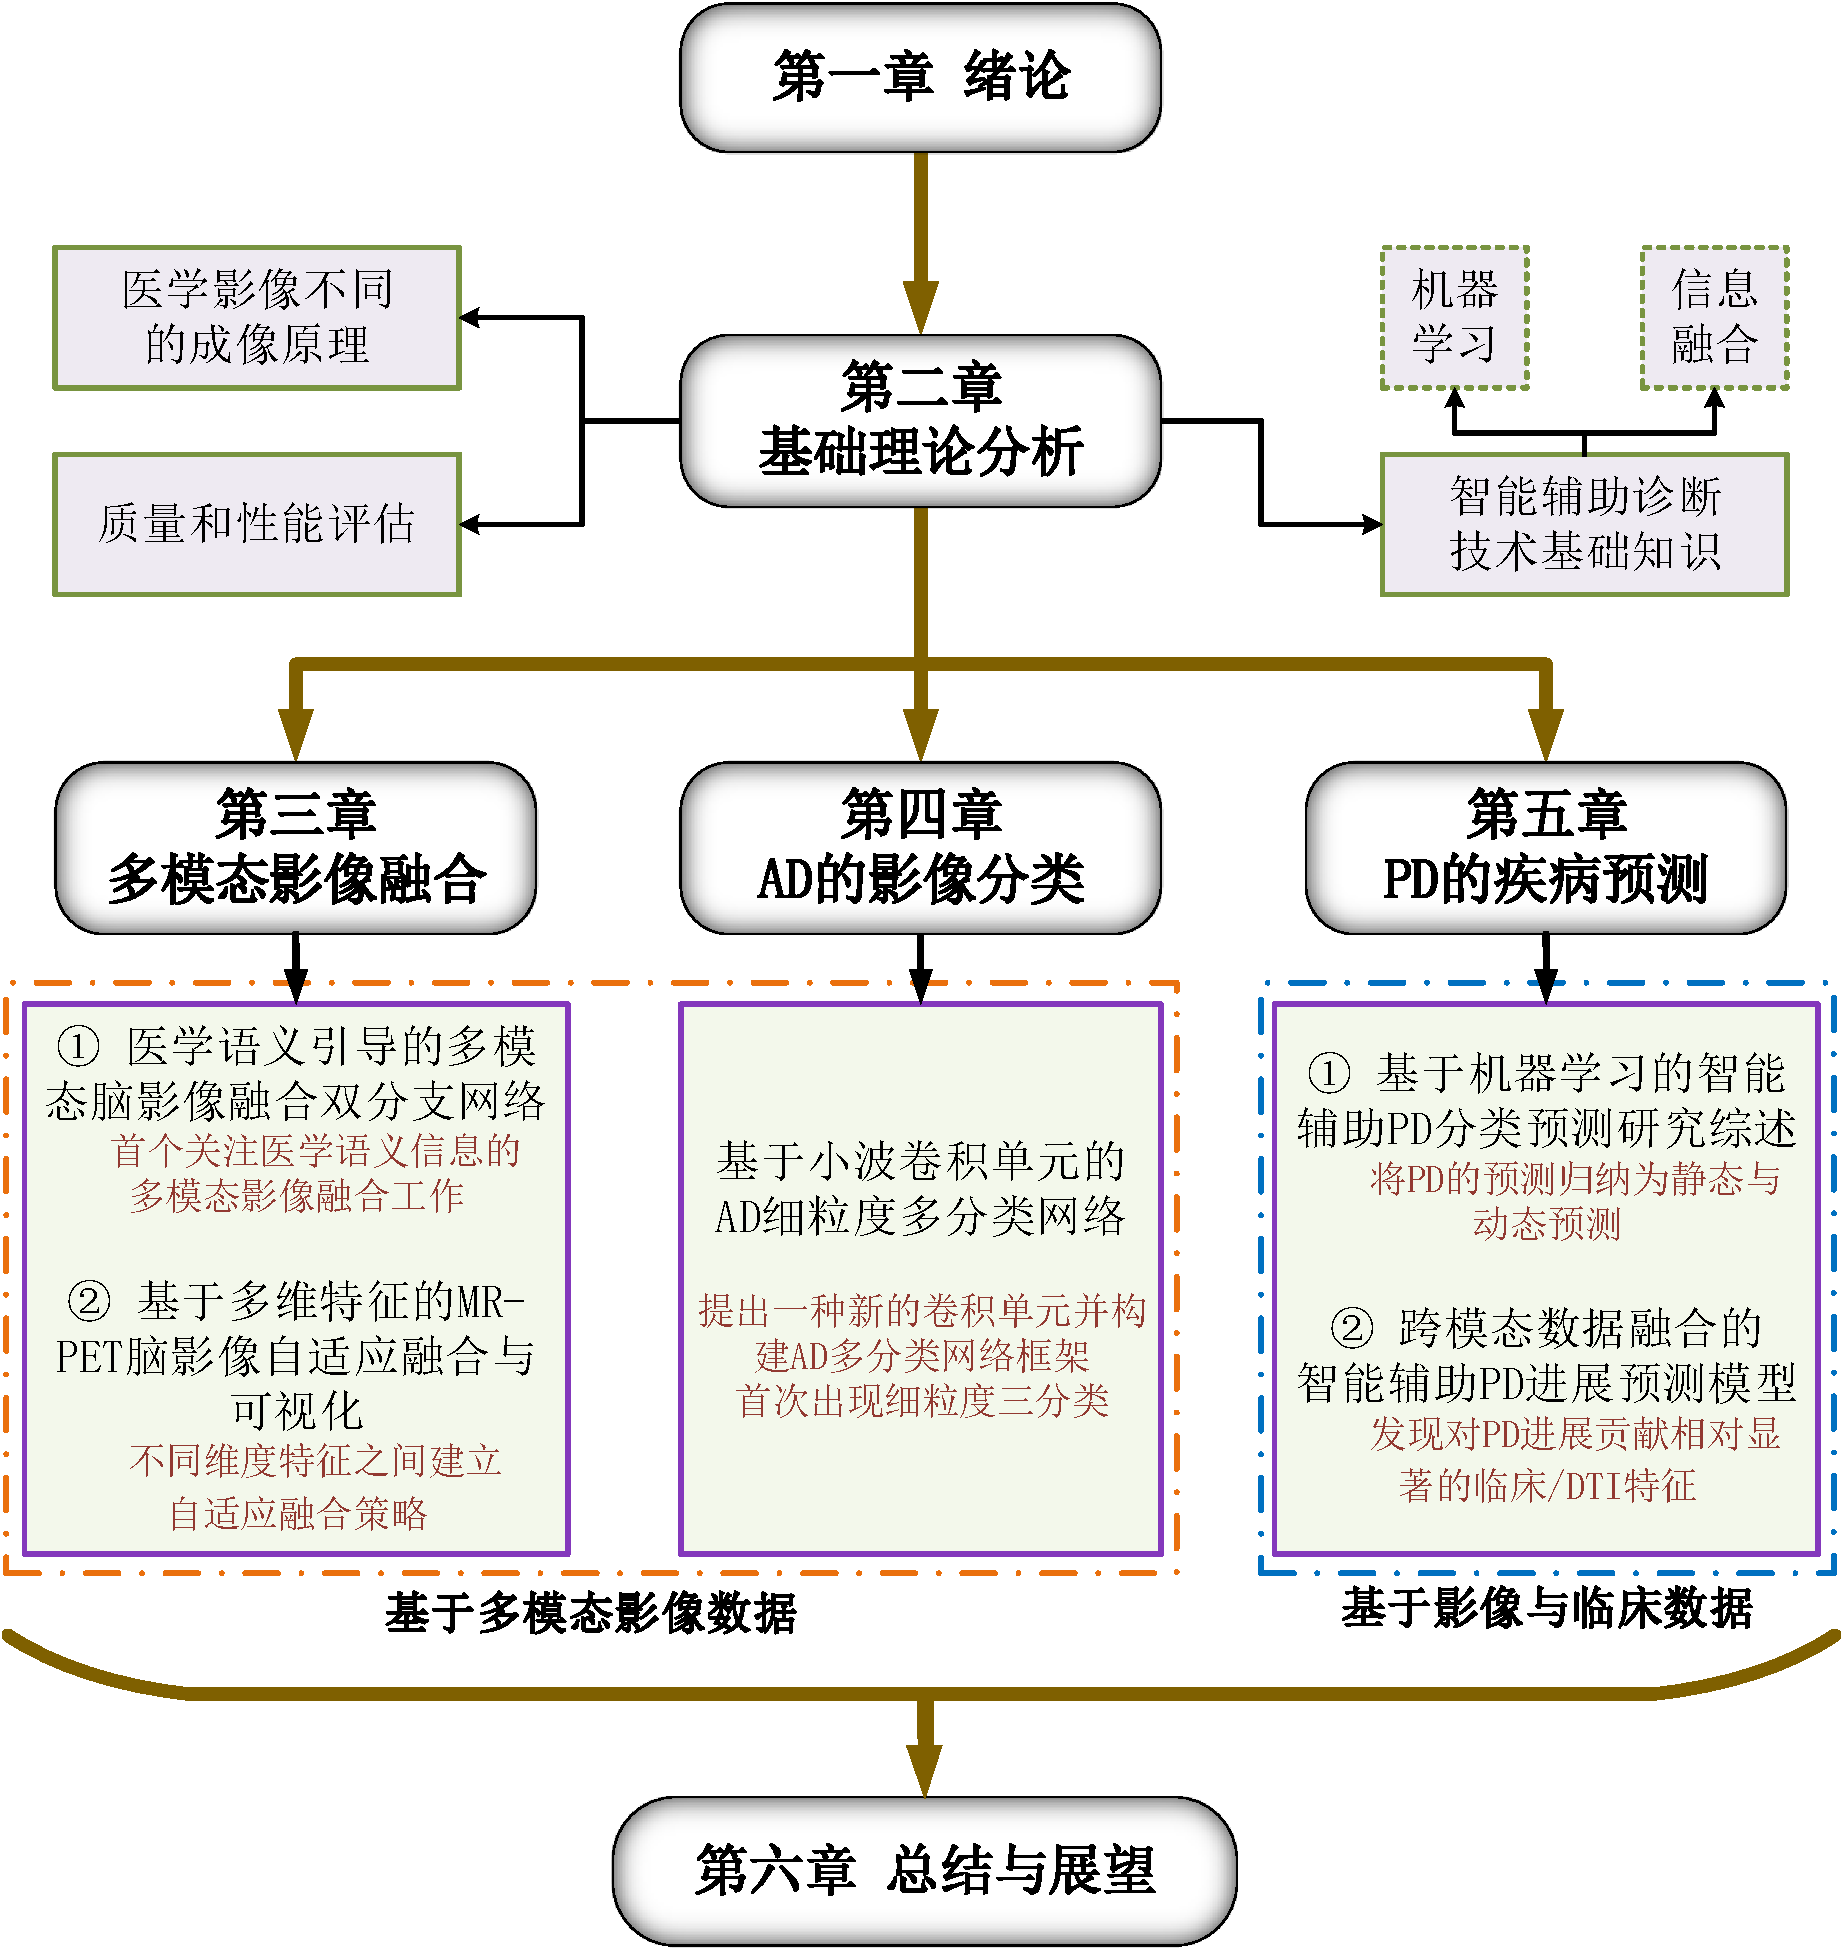
\includegraphics[width=0.88\linewidth]{figs/wholeWork.pdf}  %wholeWork.png
      \caption{本研究的内容布局与章节安排}\label{wholeWorks}
    \end{figure}

%\section{本文的篇章结构}
全文共分为六个章节,整体的篇章结构如图\ref{wholeWorks}所示。
   
第一章绪论。本章深入介绍了基于医学影像组学的智能辅助技术的研究背景与意义。强调了基于医学影像组学的智能辅助诊断技术的关键任务,包括影像融合、影像分类与疾病预测等方面。具体而言,本章详细分析了国内外在多模态医学影像融合方面的研究,包括基于传统方法和深度学习方法的不同取向。此外,本章对AD影像分类进行了深入讨论,涵盖了粗粒度分类(AD、MCI、NC的二分类或三分类)和细粒度分类(AD、EMCI、LMCI、MSC、MCI、NC的二分类、四分类和六分类)。最后,本章聚焦于PD预测,探讨了基于影像数据和基于临床数据两个层面的研究现状。整体而言,该章节不仅对研究内容进行了明晰概述,还为后续章节的深入探讨奠定了坚实基础。
    

第二章基础理论。本章深入研究了医学影像的多模态特性,对不同类型的医学影像成像技术原理进行了详细介绍,包括CT、MRI、PET等。本章详细分析了智能辅助诊断技术的理论基础,涵盖了传统机器学习方法(如SVM)和深度学习方法(如CNN)在医学影像分类中的应用。强调了这两者的融合是提高医学诊断准确性和效率的前沿趋势。另外,本章着重考虑了多模态数据的复杂性,讨论了信息融合的策略,包括像素级、特征级和决策级的融合方法,为实际应用提供了有益的启示。最后,本章还介绍了多种质量评估指标,包括主观与客观评价方法。对于有关医学影像基础理论和信息融合策略的全面认识,为后续章节中的具体技术方法提供了理论指导。


第三章聚焦于多模态影像融合。设计了两种新型的结合两种医学成像技术的融合方法,以实现更全面的信息整合。
一种是名为MsgFusion的基于医学语义信息(MS-Info)引导的融合方法。通过分析MR/CT/PET/SPECT的关键MS-Info,该方法获取相应的影像特征,采用SF分支和GV分支的双分支网络,成功提高了CNN的泛化能力。在医学脑影像的处理和分析中,包括MR-CT影像融合、MR-SPECT影像融合和MR-PET影像融合等方面,该方法相较于现有方法表现出显著优势,得到了临床医生的高度评价和统计数据的支持。
另一种也是基于深度学习的融合框架。它结合了多维特征、空间特征和通道特征,并引入了三种不同的特征提取模块(粗特征模块(coarse feature module,CFM)、精细特征模块(coarse feature module,FFM)和多尺度特征模块(multi-scale feature module,MFM))和自适应线性融合机制。该方法还提出了一种关键特征增强策略,可以增强同一病例不同时期融合影像的可视化效果,有助于肿瘤定位、分割和疾病跟踪等临床应用。
%基于本章的主要研究成果“MsgFusion: Medical Semantic Guided Two-Branch Network for Multimodal Brain Image Fusion”已在SCI Top期刊《IEEE TRANSACTIONS ON MULTIMEDIA》上刊载;“High-Quality Fusion and Visualization for MR-PET Brain Tumor Images via Multi-Dimensional Features”已收到SCI Top期刊《IEEE TRANSACTIONS ON IMAGE PROCESSING》的录用通知。


第四章关注AD影像分类。首先,提出了一种创新的卷积单元(wavelet convolution unit,WCU),它将小波变换与传统卷积函数结合,以获得更广泛的非局部感受野,显著提升卷积神经网络性能。在WCU的引导下,本章设计了影像分类的网络框架(WCU-Net)成功应用于AD的细粒度和多分类任务。基于AD的脑DTI数据(NC、MCI、EMCI、LMCI、AD)实现了所有粗粒度和细粒度的12种组合分类,包括首次引入的细粒度三分类。该框架在所有12种分类中取得了高准确率,尤其在8种细粒度分类中表现卓越。细粒度四分类的准确率仍有提升空间,并计划未来将WCU-Net应用于不同疾病的分类和分期。
%基于本章的主要研究成果“Fine-Grained and Multiple Classification for Alzheimer’s Disease With Wavelet Convolution Unit Network”已在SCI期刊《IEEE TRANSACTIONS ON BIOMEDICAL ENGINEERING》上刊载。


第五章探讨PD疾病预测。
首先,本章详细回顾了基于机器学习的PD分类预测的研究。全面介绍了静态和动态两种研究方法,而且突出了机器学习在增强PD智能辅助诊断和健康评估中的巨大应用前景。本章深入分析了在PD预测中所采用的数据类型,并探讨了PD预后领域未来的发展潜力和可能的演变路径。
其次,本章提出了一种基于跨模态数据融合的智能辅助PD进展预测的新方法(CMFP)。它通过集成基线DTI和临床特征数据,该方法的独特之处在于采用纵向数据研究方法,结合机器学习技术,建立了早期PD基线DTI及临床特征的疾病进展模型。研究结果显示,跨模态数据融合显著提升了单模态预测的准确度,并且DTI数据对临床预测性能的提升具有显著作用。这一发现为未来的PD研究指明了方向,强调了跨模态数据融合在提高预测性能方面的潜在优势。
%基于本章的主要研究成果“基于机器学习的智能辅助帕金森疾病分类预测研究综述”已在中文核心期刊《图学学报》上刊载。“Prediction of Parkinson’s disease progression based on cross-modal fusion of DTI and clinical data”已投稿至SCI期刊《npj Parkinsons Disease》。

第六章回顾总结了全文研究内容,阐述了在当前研究工作中所存在的不足,并展望了未来可能的研究方向和工作设想,为基于医学影像组学的智能诊断技术发展提供了实践经验和研究思路。